%%%%%%%%%%%%%%%%%%%%%%%%%%%%%%%%%%%%%%%%%%%%%%%%%%%%%%%%%%%%%%%%%%%%%%%%%%%%%%%%
%2345678901234567890123456789012345678901234567890123456789012345678901234567890
%        1         2         3         4         5         6         7         8

%\documentclass[a4paper, 10 pt, conference]{ieeeconf}  % Comment this line out if you need a4paper

\documentclass[letterpaper, 10pt, conference]{ieeeconf}      % Use this line for a4 paper

\IEEEoverridecommandlockouts                              % This command is only needed if 
                                                          % you want to use the \thanks command

\overrideIEEEmargins                                      % Needed to meet printer requirements.

%In case you encounter the following error:
%Error 1010 The PDF file may be corrupt (unable to open PDF file) OR
%Error 1000 An error occurred while parsing a contents stream. Unable to analyze the PDF file.
%This is a known problem with pdfLaTeX conversion filter. The file cannot be opened with acrobat reader
%Please use one of the alternatives below to circumvent this error by uncommenting one or the other
%\pdfobjcompresslevel=0
%\pdfminorversion=4

% See the \addtolength command later in the file to balance the column lengths
% on the last page of the document

% The following packages can be found on http:\\www.ctan.org
%\usepackage{graphics} % for pdf, bitmapped graphics files
%\usepackage{epsfig} % for postscript graphics files
%\usepackage{mathptmx} % assumes new font selection scheme installed
%\usepackage{times} % assumes new font selection scheme installed
%\usepackage{amsmath} % assumes amsmath package installed
%\usepackage{amssymb}  % assumes amsmath package installed
\usepackage{textcomp}
\usepackage{xurl}
\usepackage{amsmath,bm}
\usepackage{amssymb}
\usepackage{graphicx}
\usepackage{subcaption}
\usepackage{siunitx}
\usepackage{cite}
\usepackage{psfrag}
\usepackage{multirow}
\usepackage{flushend}

\renewcommand\vec{\mathbf}

\title{\LARGE \bf
On the 3D trochoidal motion model of LiDAR sensors\\placed off-centered inside spherical mobile mapping systems
}

\author{Fabian Arzberger$^{1}$ and Andreas N{\"u}chter$^{1}$% <-this % stops a space
\thanks{$^{*}$We acknowledge funding from the Elite Network Bavaria (ENB) for providing funds for the academic program ``Satellite Technology''}% <-this % stops a space
\thanks{$^{1}$The authors are with Computer Science XVII -- Robotics,
        Julius-Maximilians-Universit{\"a}t W{\"u}rzburg, 97074 Am Hubland, Germany.
        {Contact: \tt\small fabian.arzberger@uni-wuerzburg.de}}%
}


\begin{document}



\maketitle
\thispagestyle{empty}
\pagestyle{empty}


%%%%%%%%%%%%%%%%%%%%%%%%%%%%%%%%%%%%%%%%%%%%%%%%%%%%%%%%%%%%%%%%%%%%%%%%%%%%%%%%
\begin{abstract}
We study the motion model of a sensor rigidly mounted inside a ball.
Due to the rigid placement inside the ball, the geometry of the sensor trajectory resembles a 3D curate trochoid.
A new calibration method for spherical systems estimates the extrinsic parameters of the sensor with respect to the balls center of rotation.
We deploy the calibration and motion model on our spherical mobile mapping platform to estimate the trajectory of a LiDAR sensor and compare it to trajectories of state-of-the-art LiDAR-Inertial odometry (LIO) methods.
The motion model, which is solely based on IMU measurements, produces comparable results to the LIO methods, sometimes even outperforming them in positional accuracy.
Although the LIO methods provide better rotational accuracy due to the utilization of LiDAR data, they struggle to reproduce the trochoidal nature of the trajectory and only provide pose estimations at the LiDAR frequency, whereas the motion model produces a more consistent trochoidal trajectory at the much higher IMU frequency.
The results demonstrate the difficulty that current LIO methods have on spherical systems and indicate that our motion model is suitable for overcoming these issues. 
\end{abstract}

\section{Introduction}


% \begin{figure}
%   \centering 
%   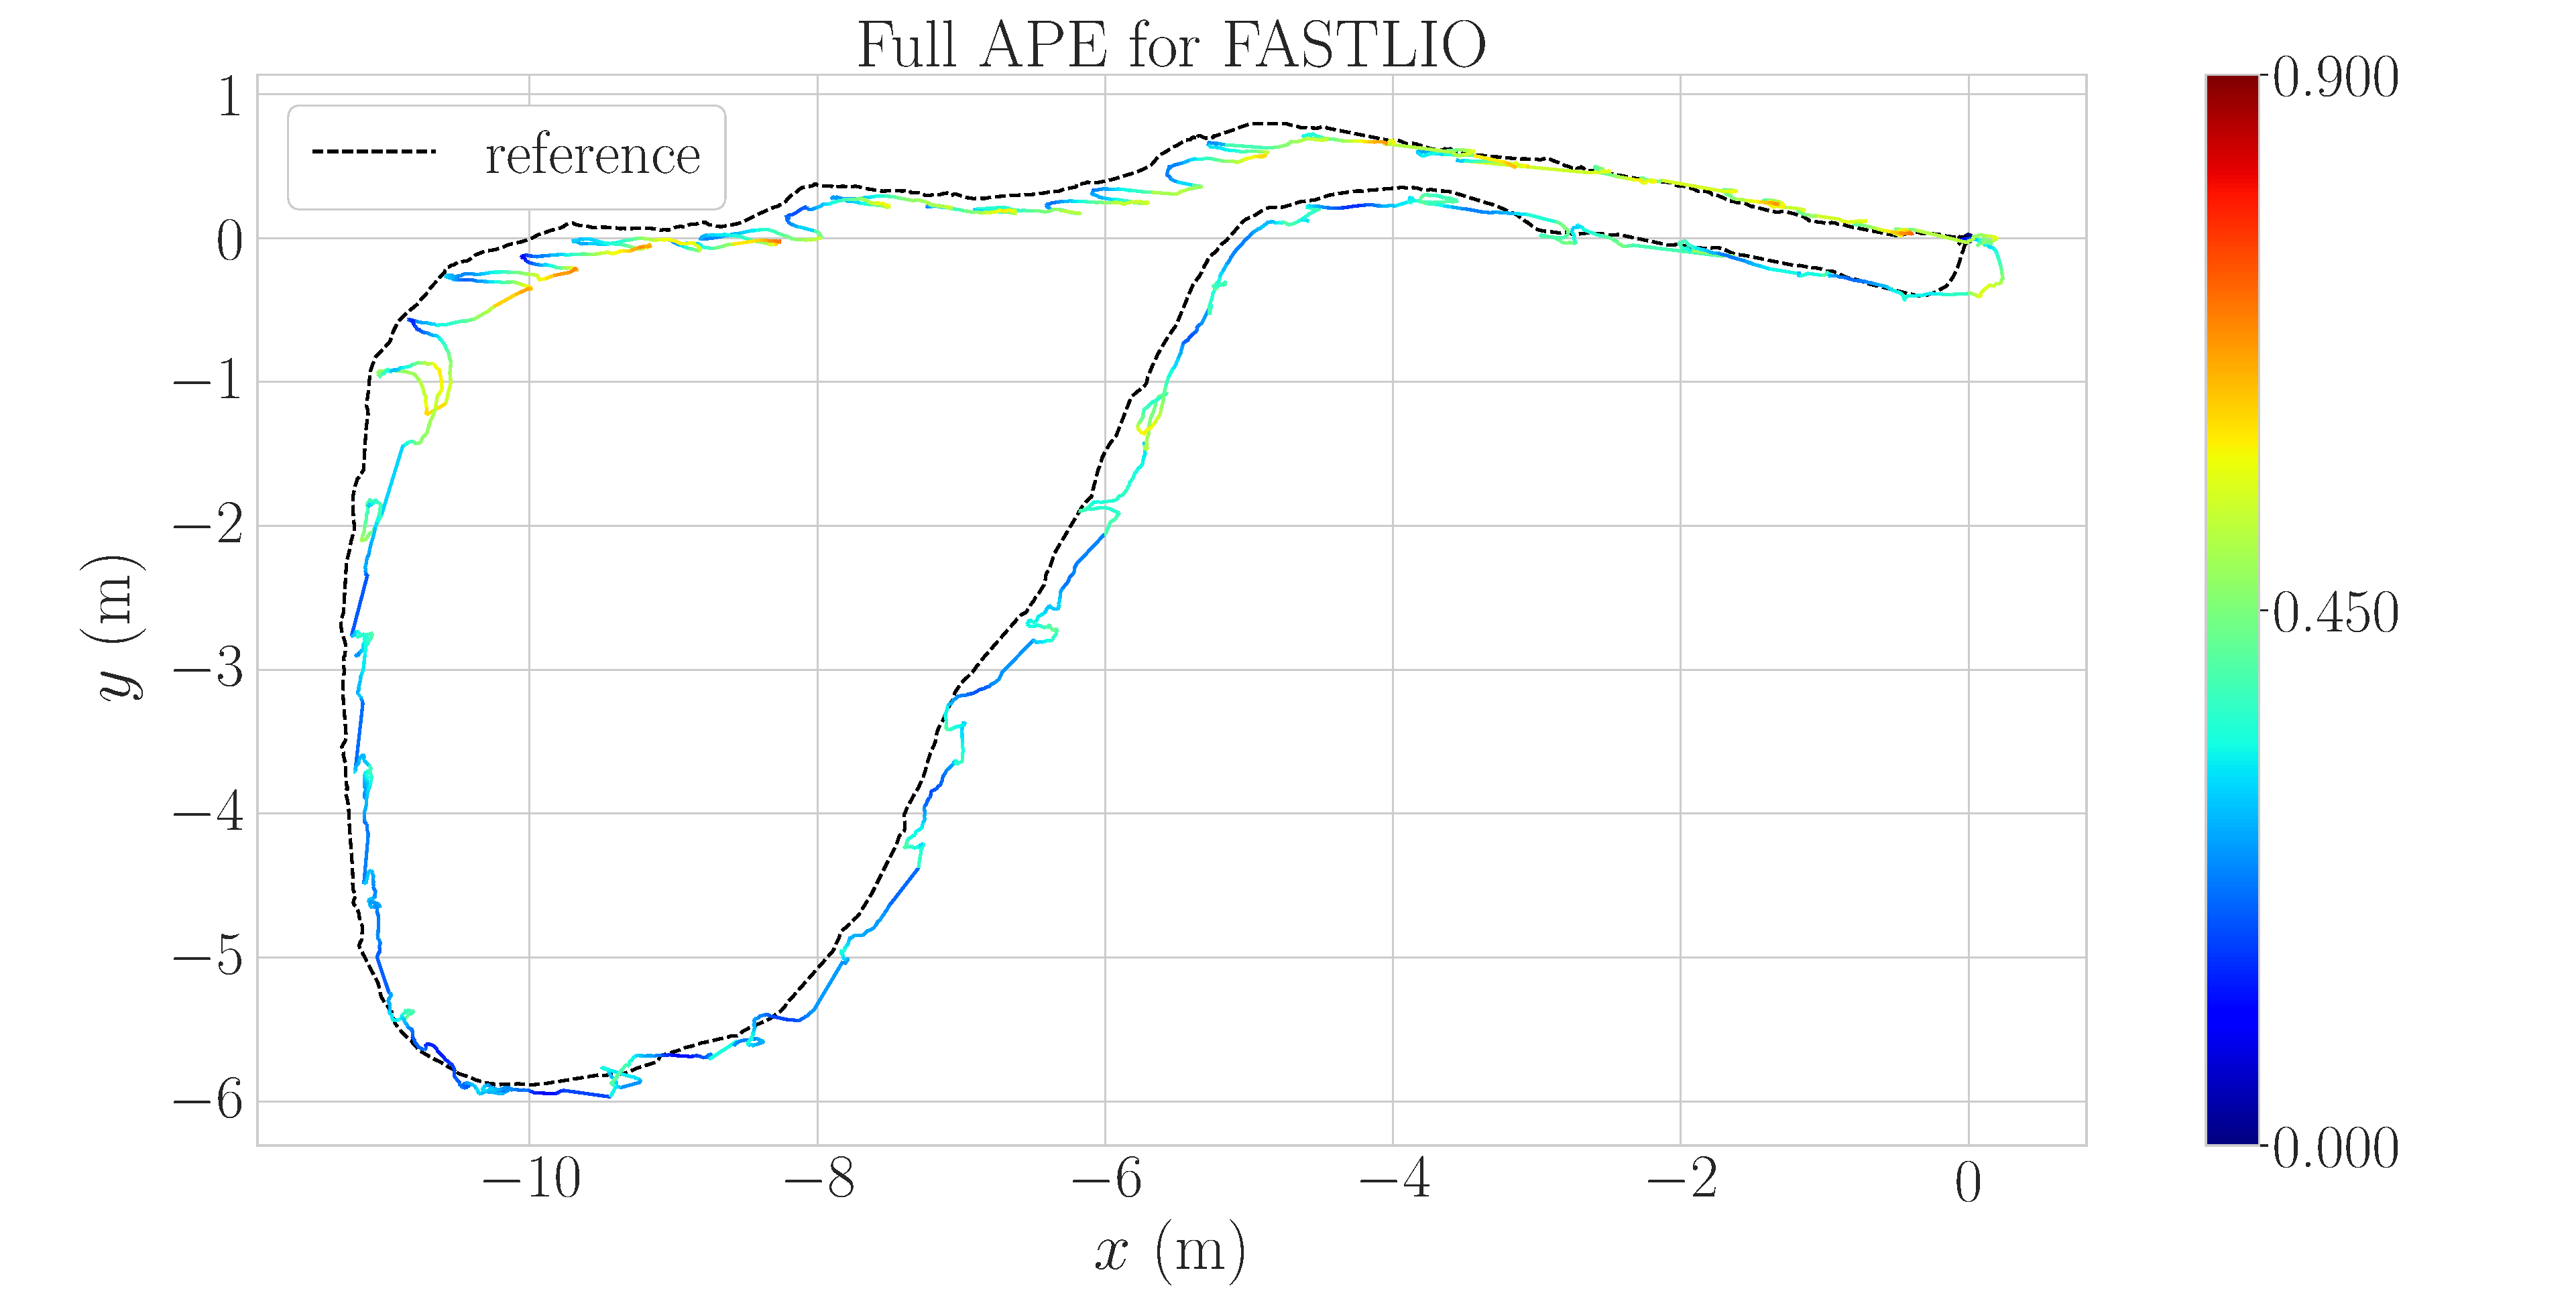
\includegraphics[width=\linewidth]{img/ape_fast_lio} \vskip 2mm
%   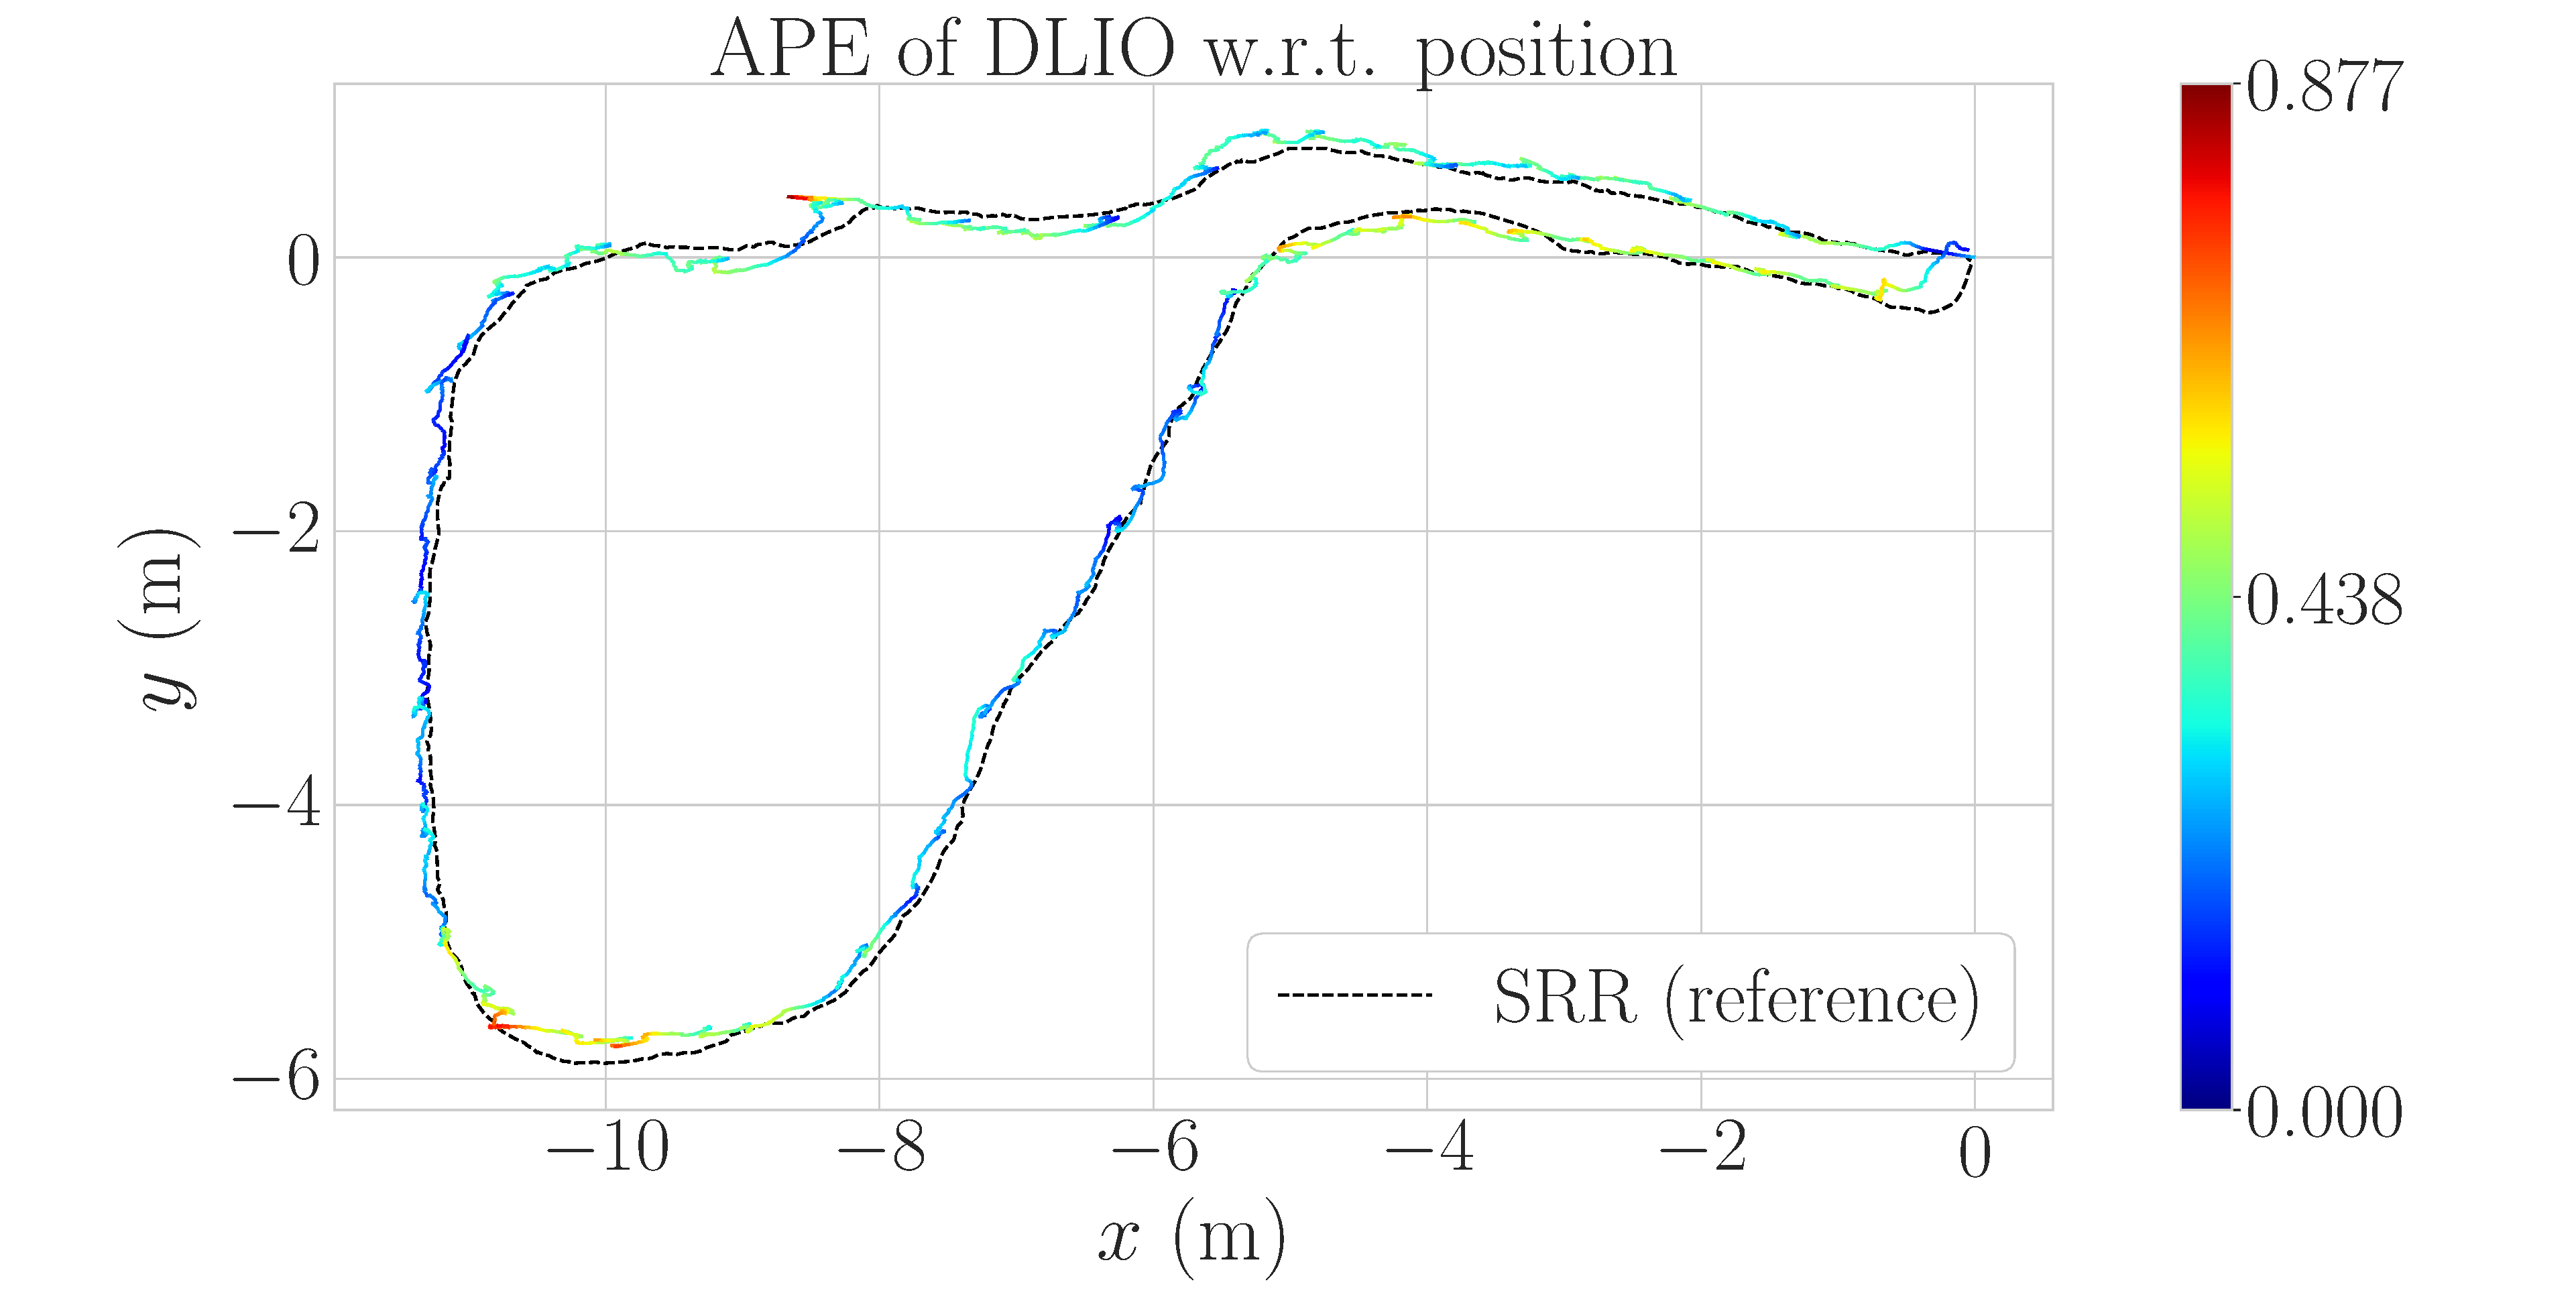
\includegraphics[width=\linewidth]{img/ape_dlio} \vskip 2mm
%   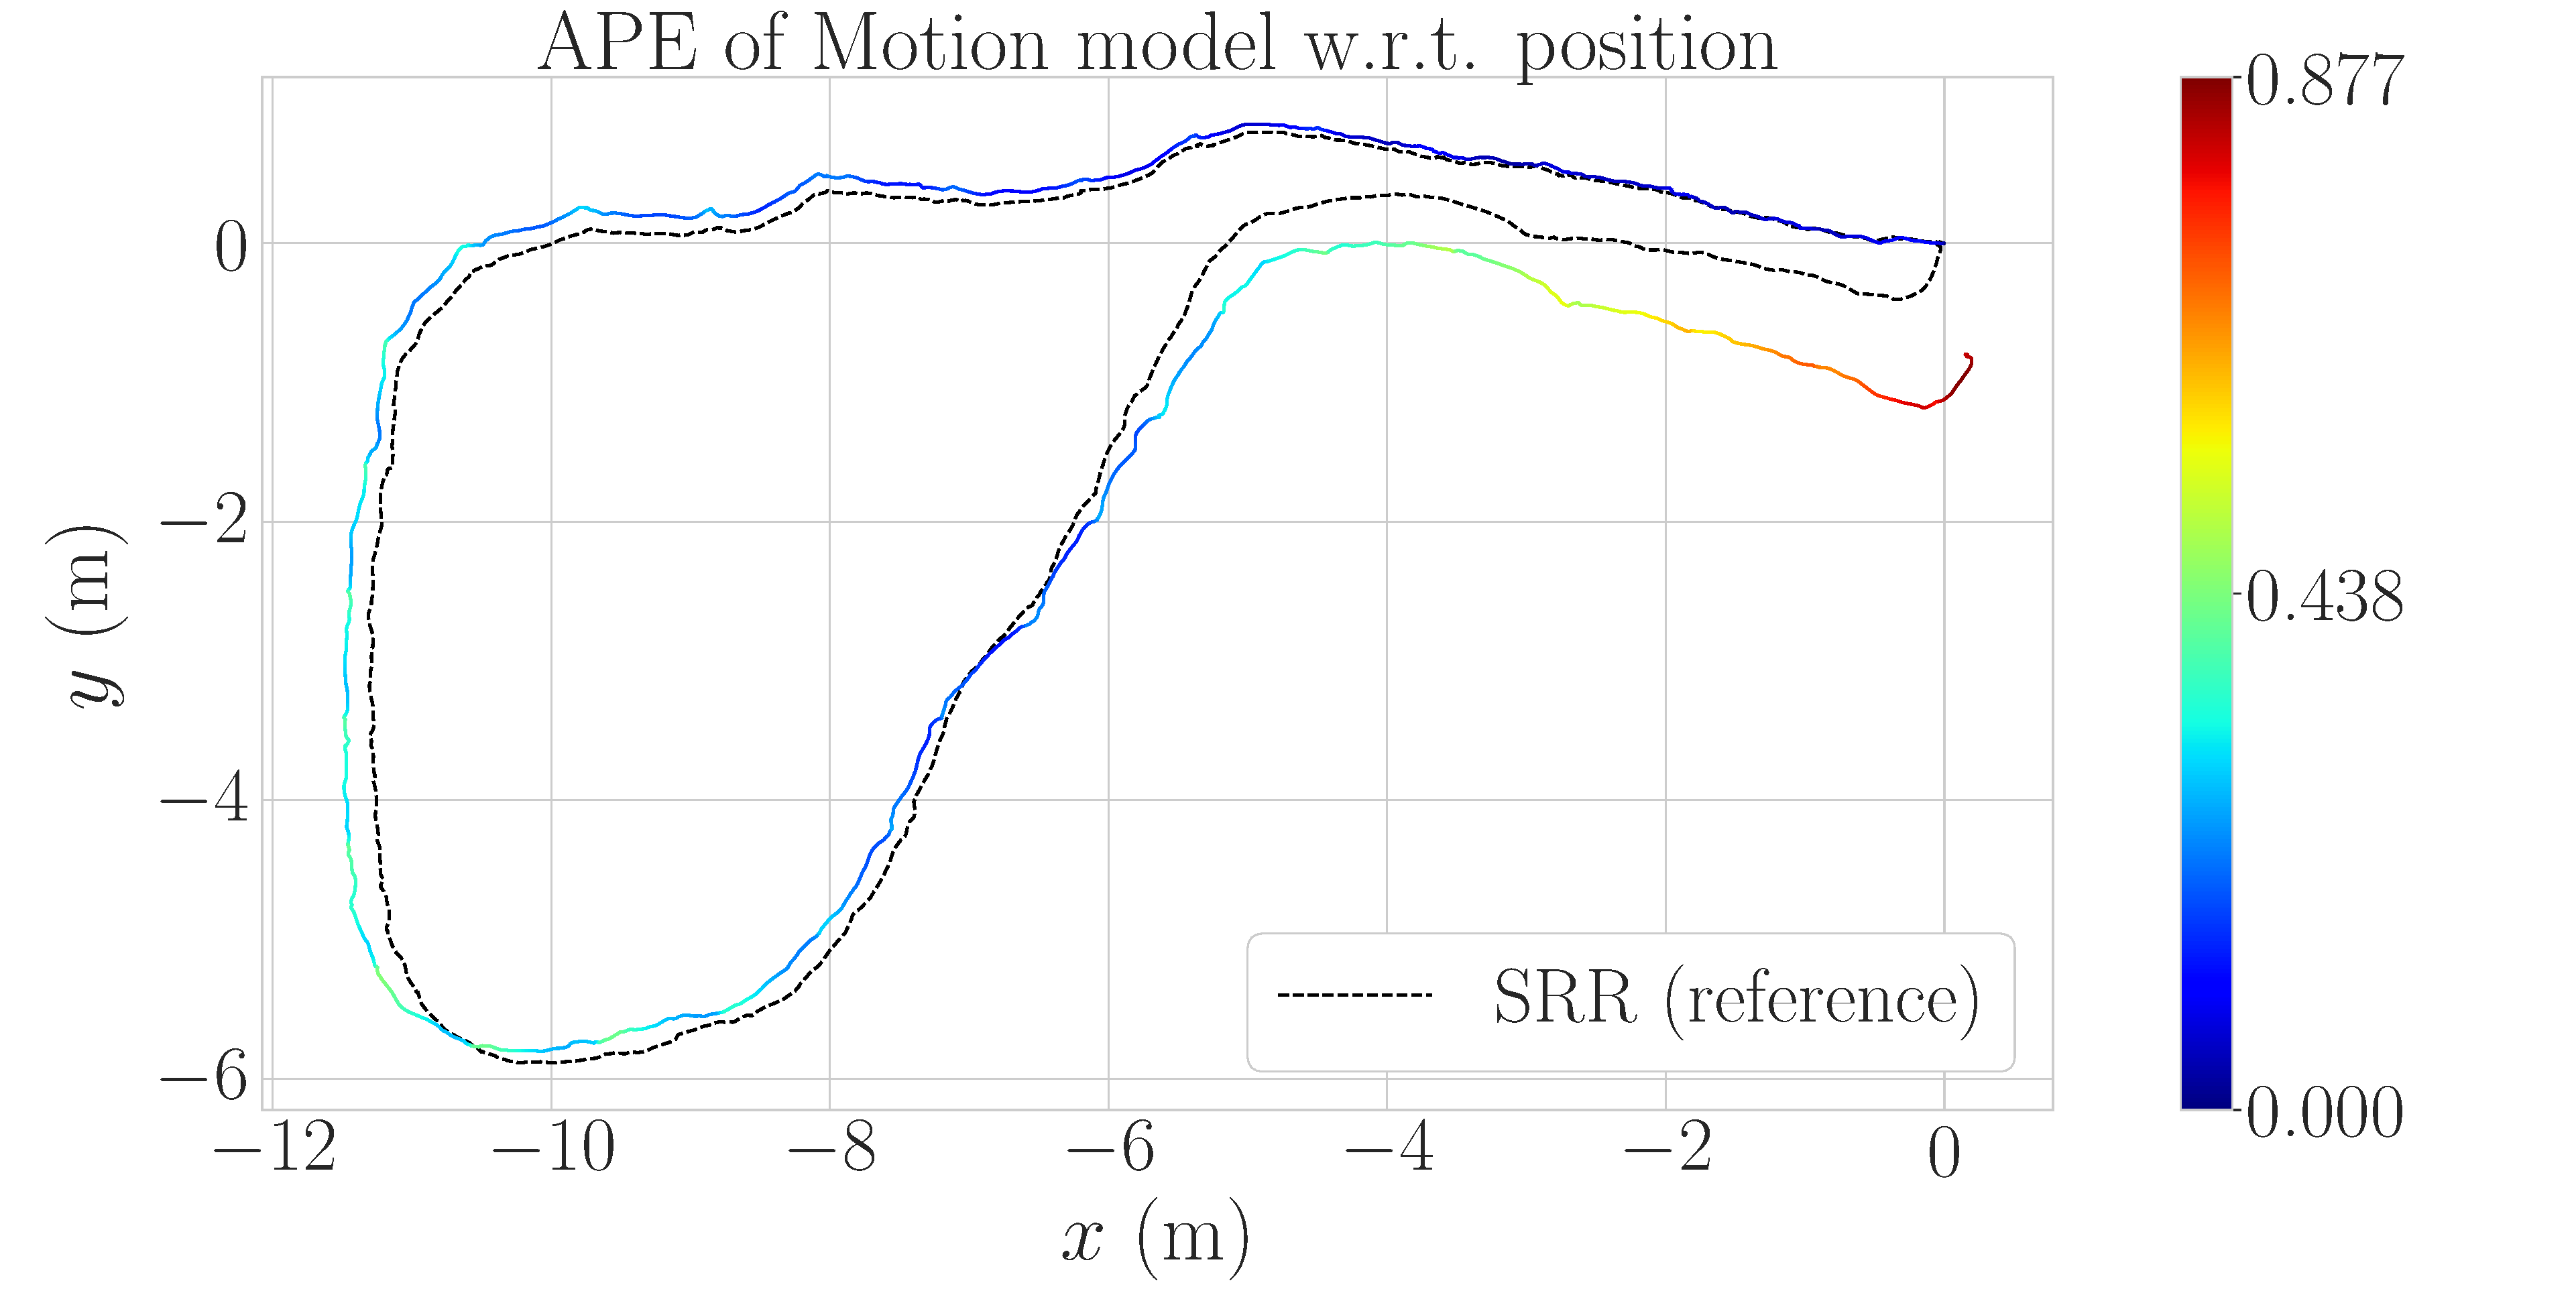
\includegraphics[width=\linewidth]{img/ape_model}
%   \caption{Tripple caption.}
%   \label{fig:ape}
% \end{figure}

% \begin{figure}
%   \centering 
%   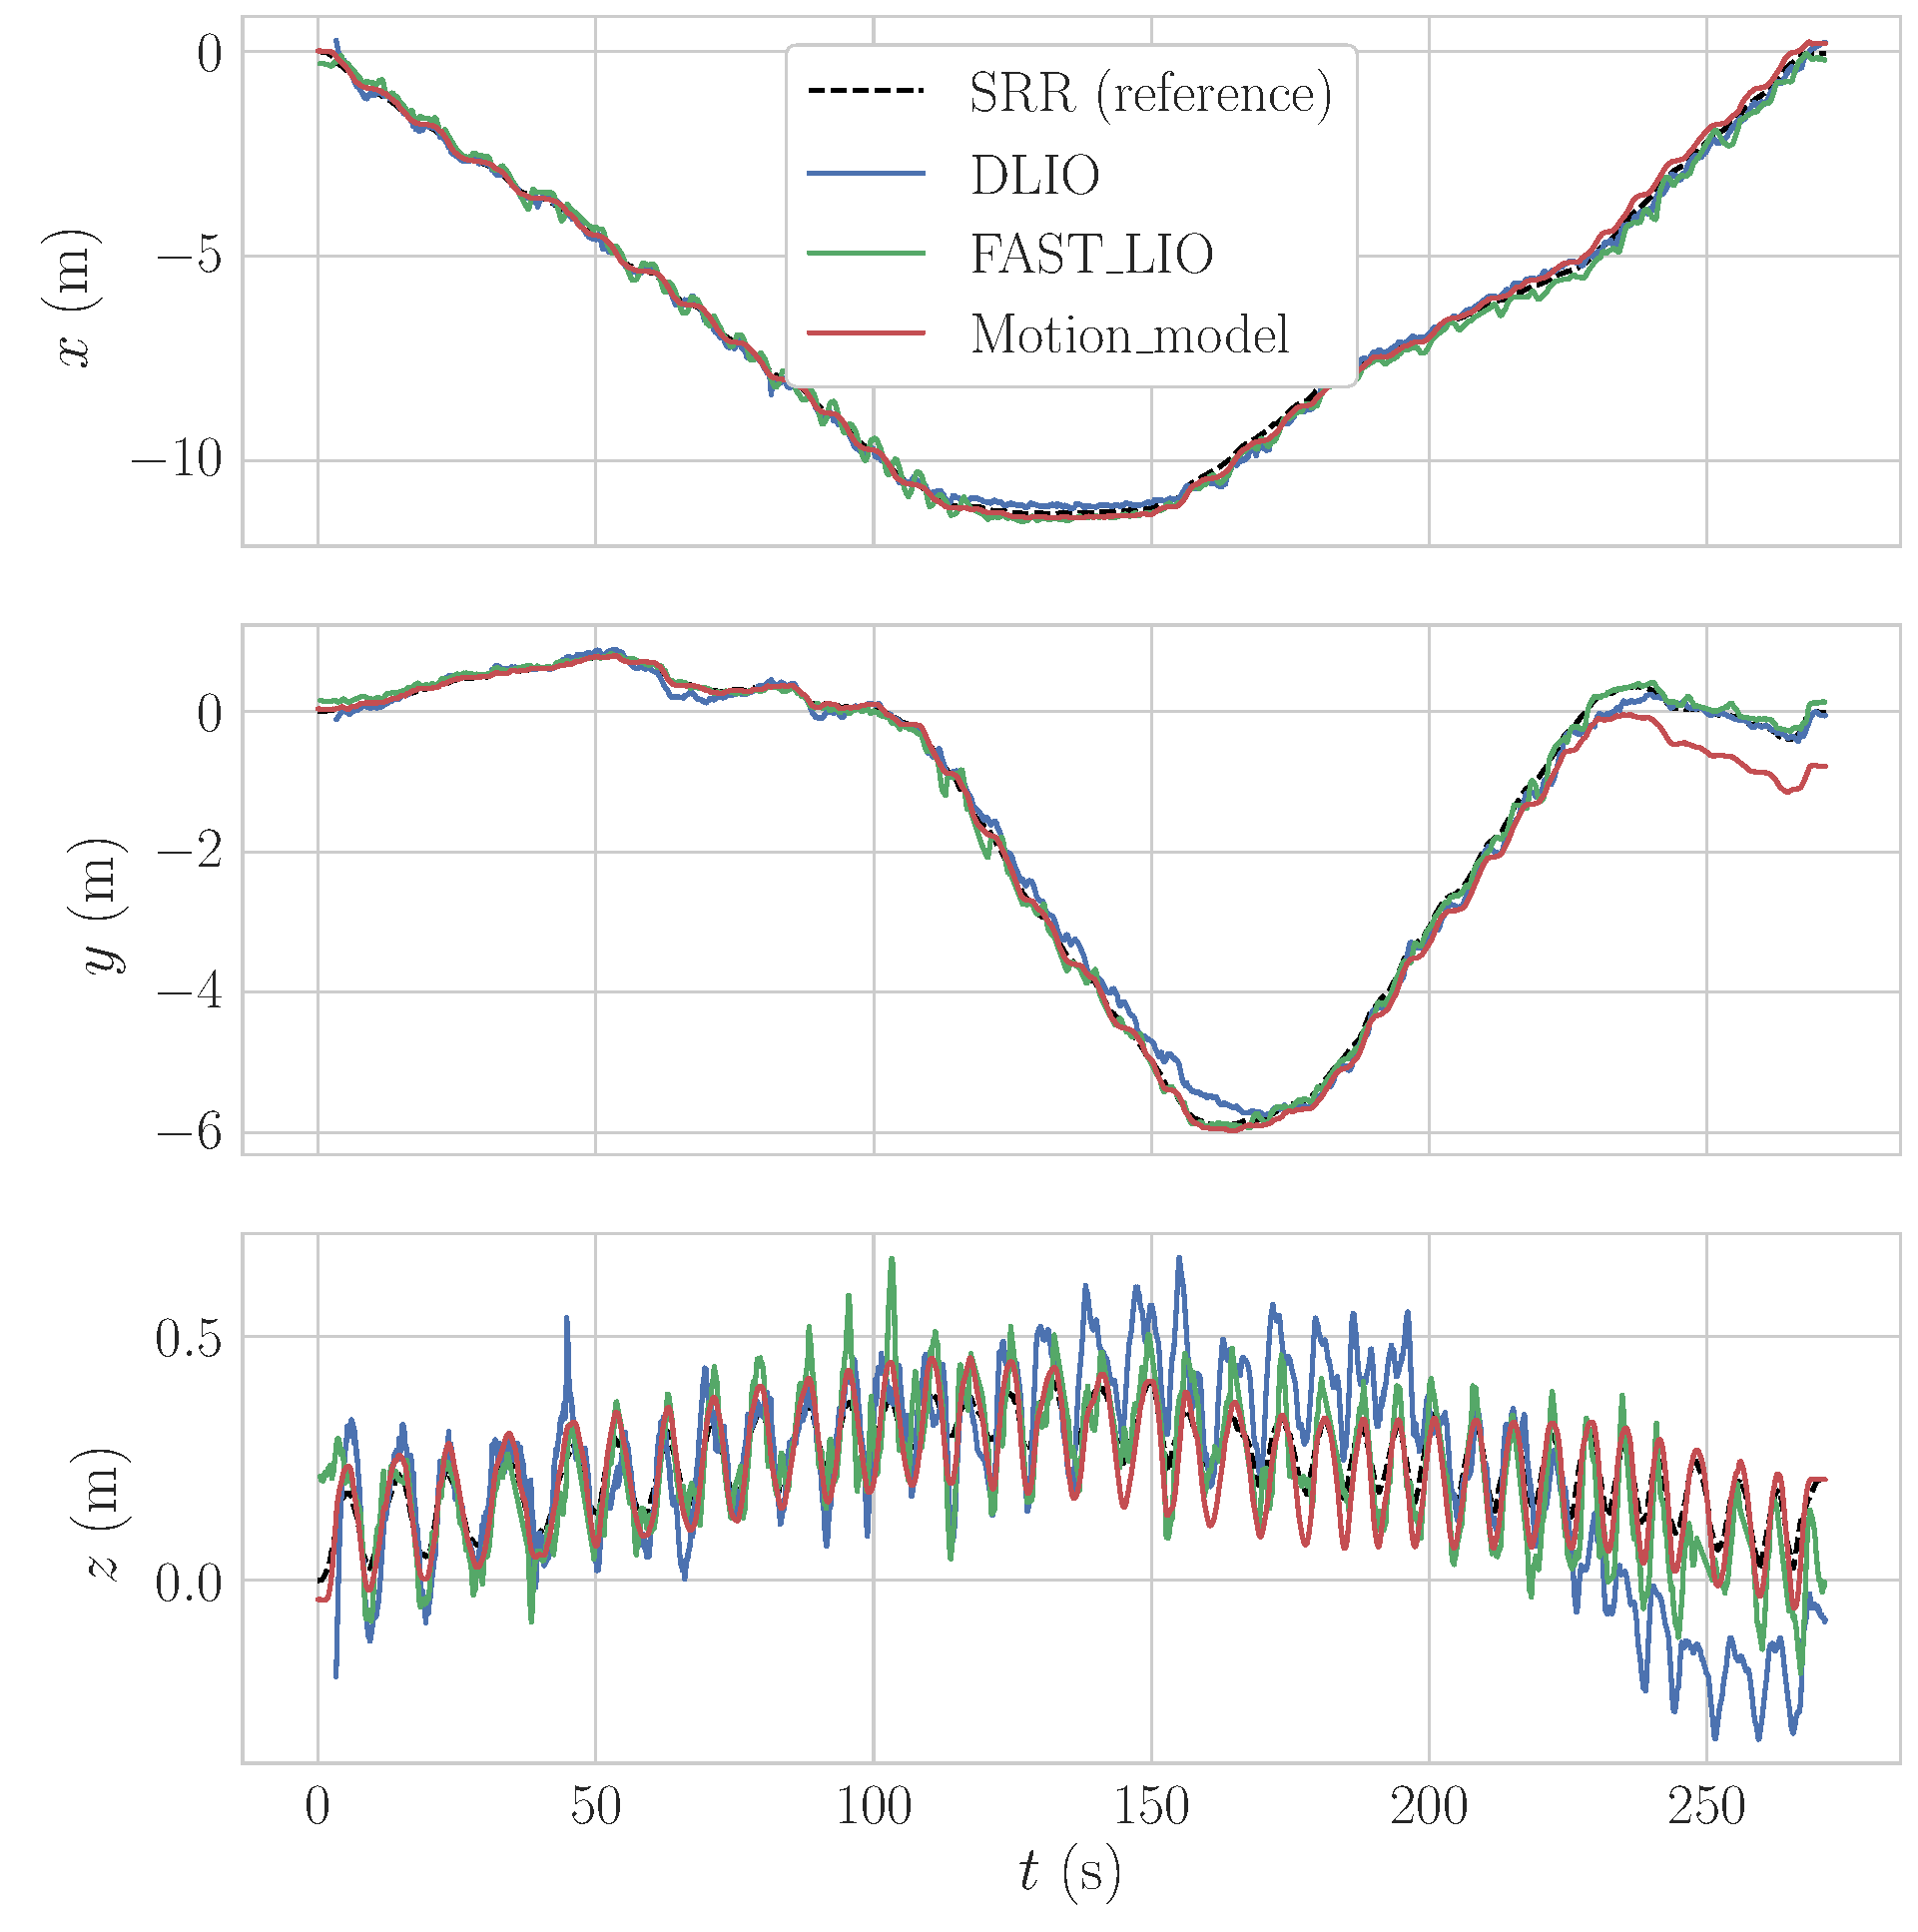
\includegraphics[width=\linewidth]{img/trajectory_components}
%   \caption{Another caption.}
%   \label{fig:components}
% \end{figure}


\section{Related work}
\begin{figure}
  \centering 
  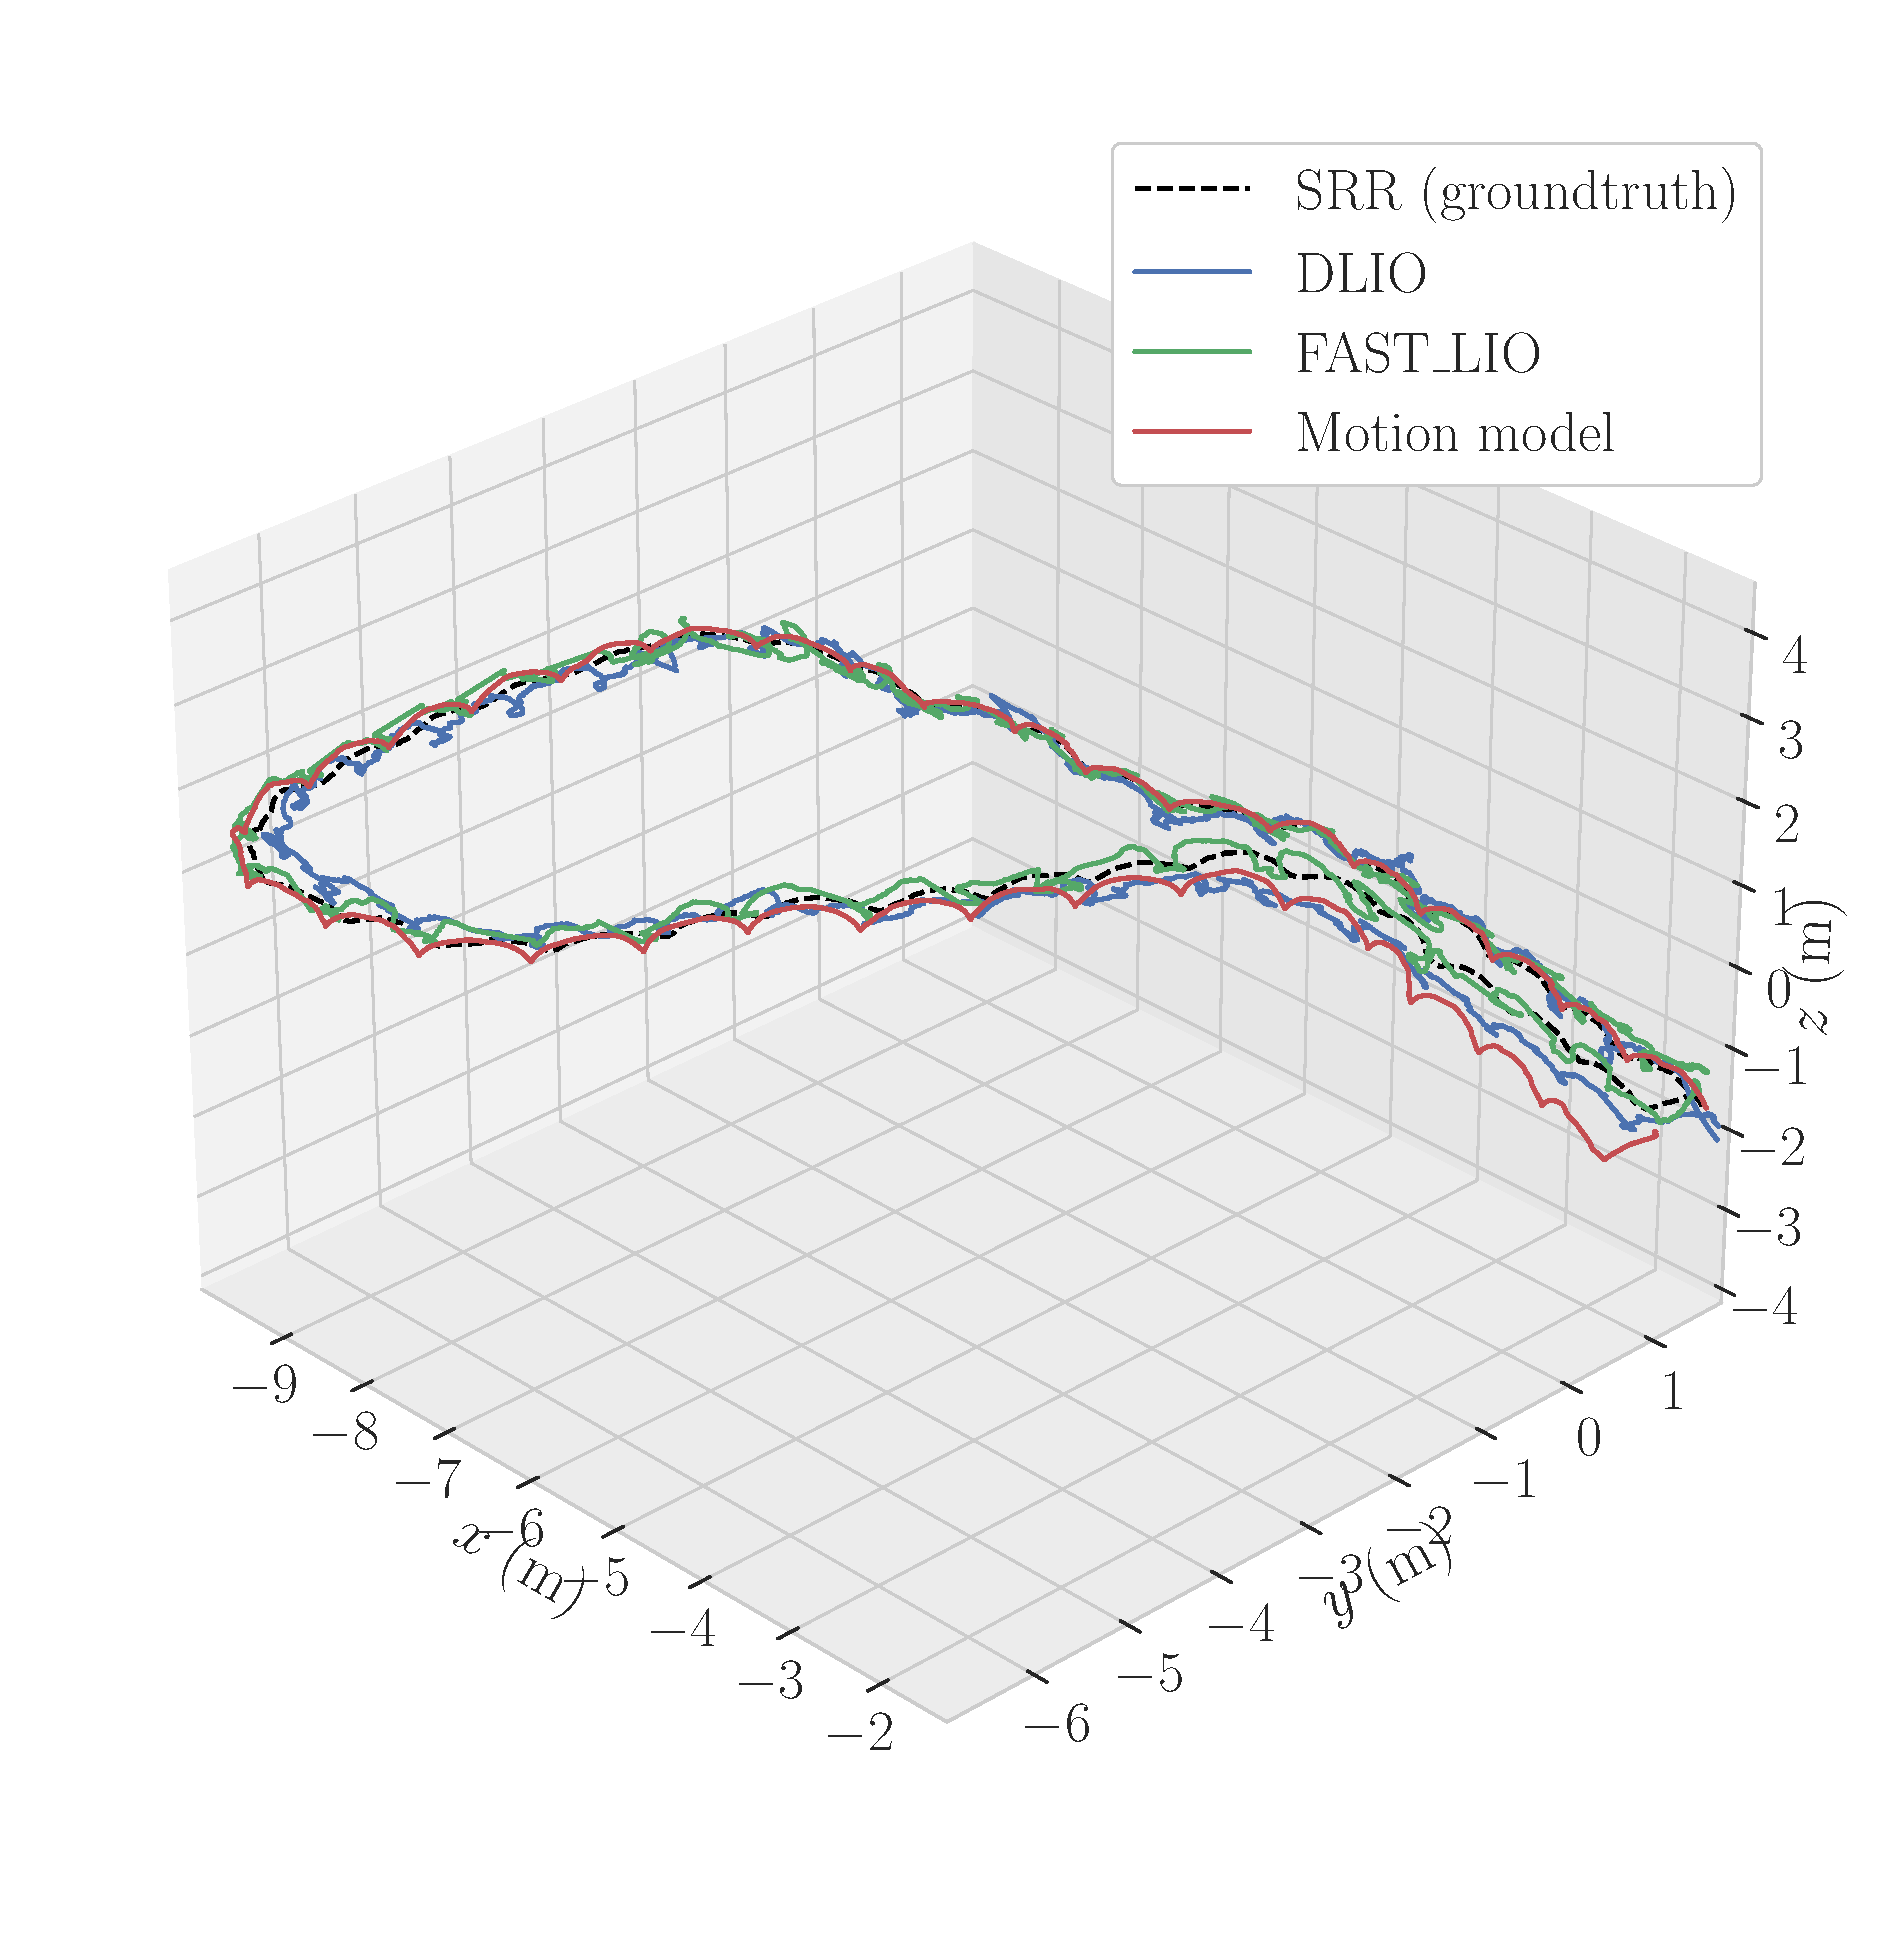
\includegraphics[width=\linewidth]{img/trajectory_3d}
  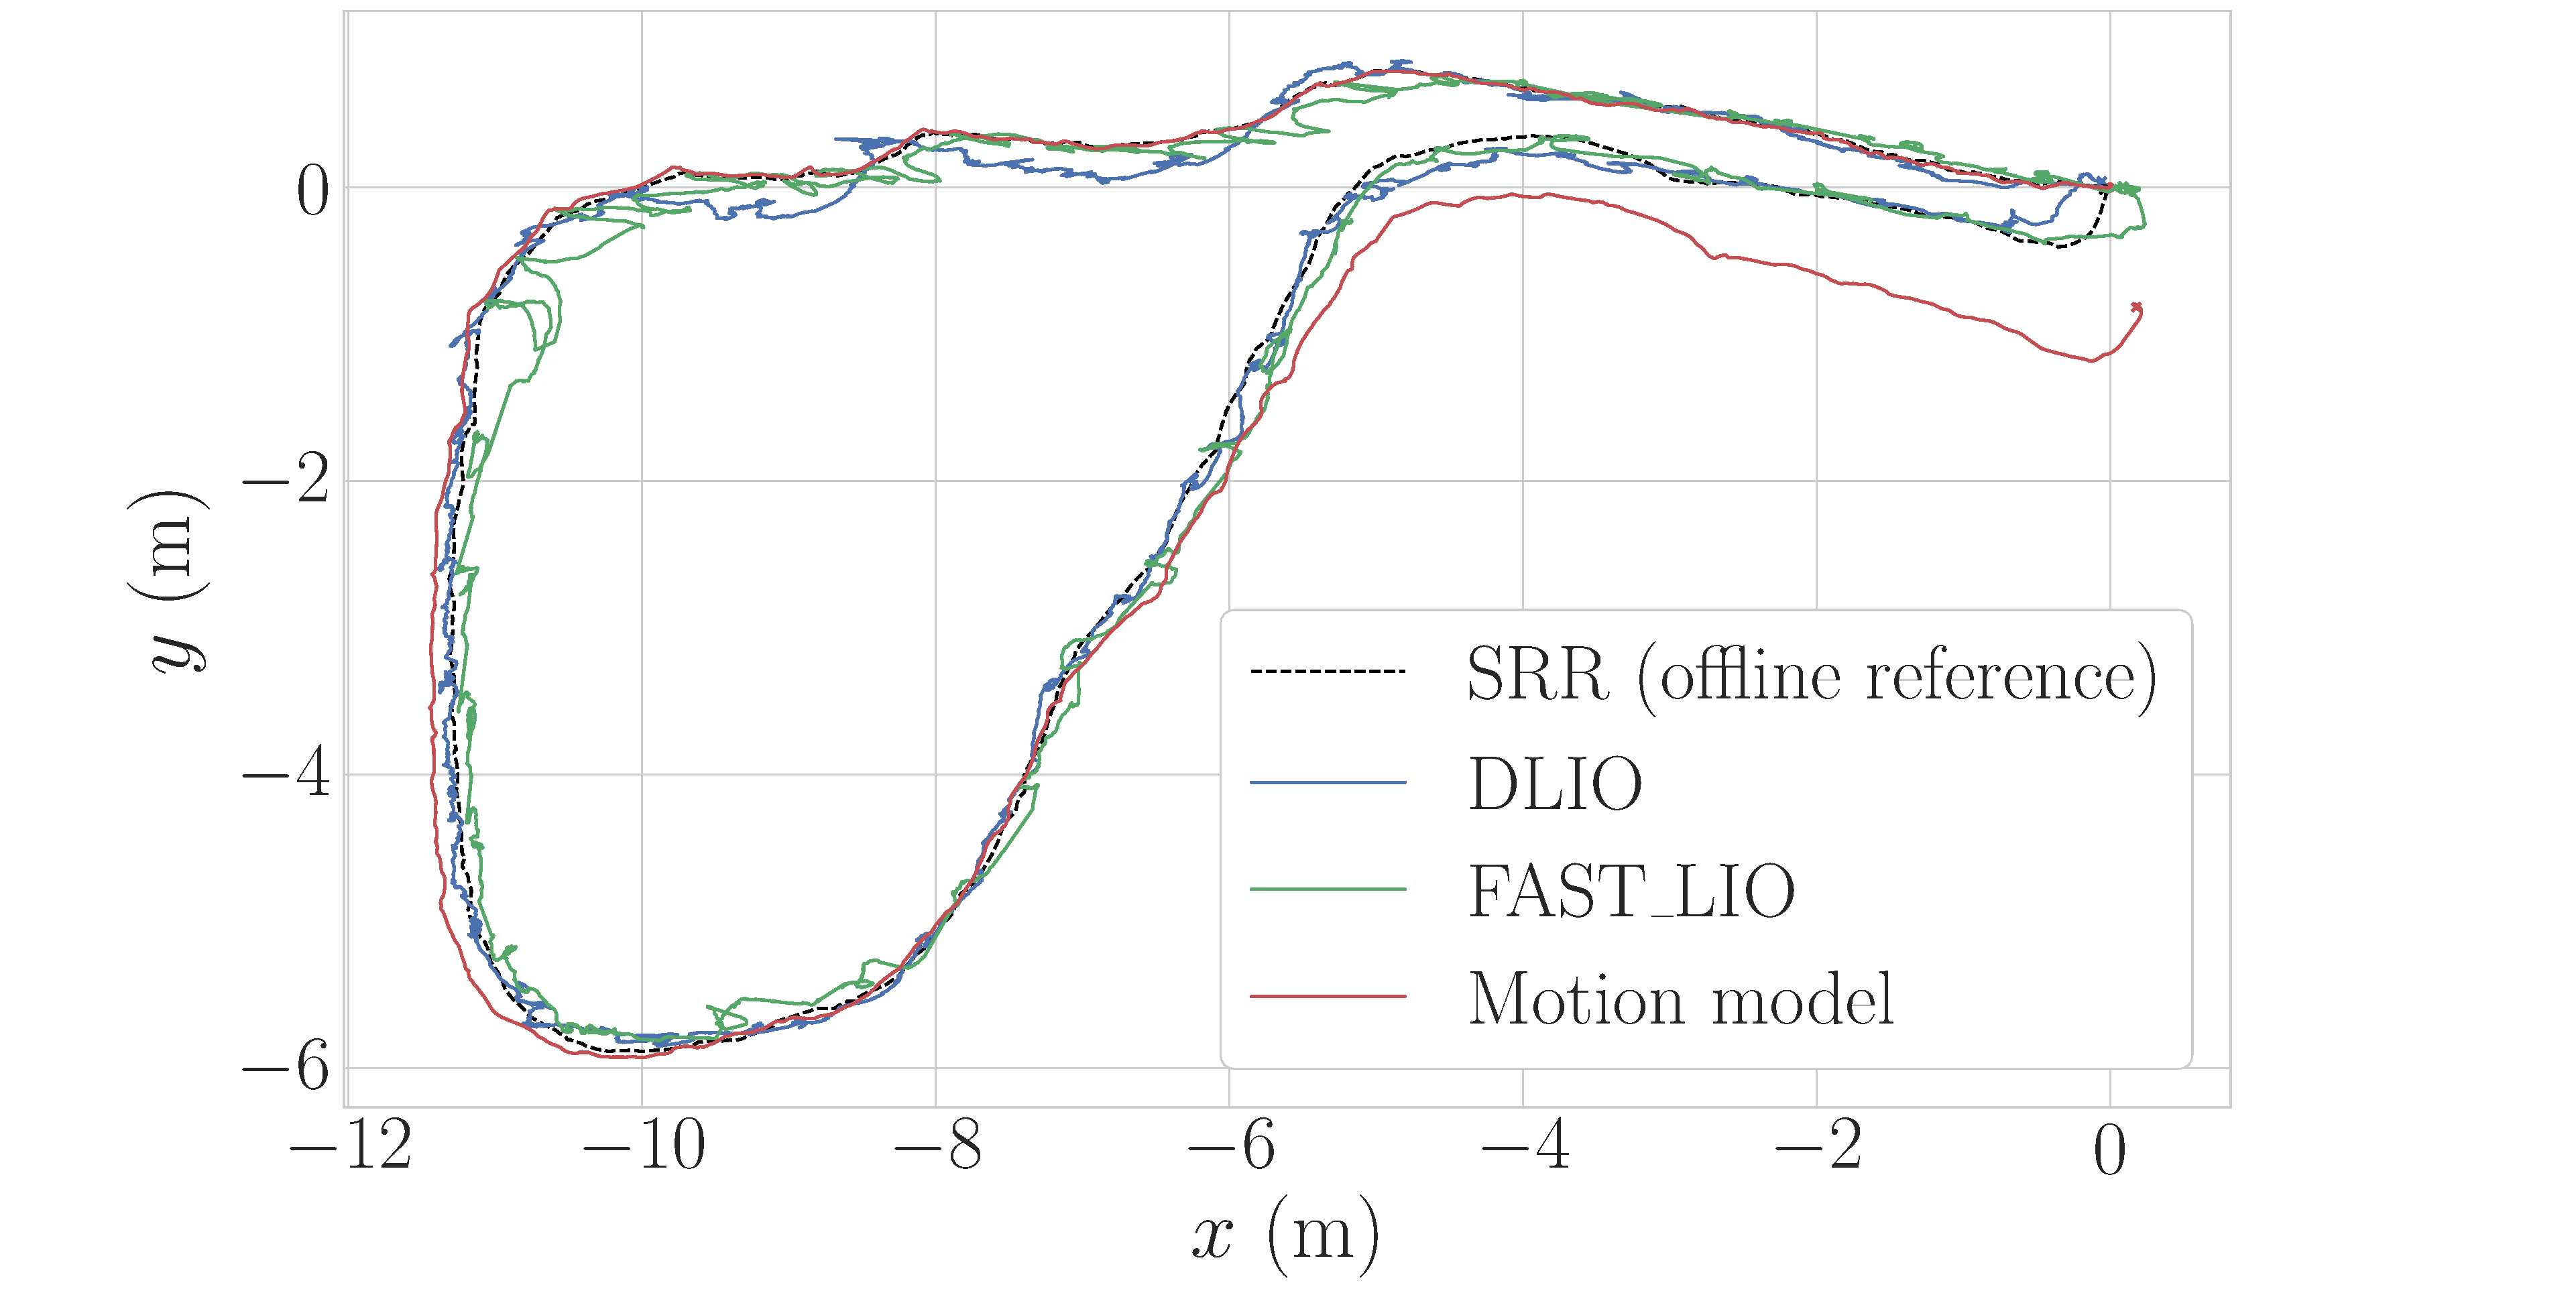
\includegraphics[width=\linewidth]{img/trajectory_xy}
  \caption{A caption.}
\end{figure}
\section{Extrinsic calibration}

\begin{figure}[h]
  \centering
  \includegraphics[width=.5\linewidth]{img/calibsphere}
  \caption{Calibration principle of a sensor inside a ball, illustrated in one axis.}
  \label{fig:calibsphere}
\end{figure}

The sensor, when mounted off-centered in the ball, will make circular trajectories if the ball rotates around an axis through its center.
We measure the radii of the sensor around the three orthogonal principal axes, which is enough information to construct the extrinsic parameters, describing the offset to the balls center.
\section{Trochoidal motion model}

\begin{figure*}
  \centering
  \includegraphics[width=.8\textwidth]{img/schematics}
  \caption{Schematics of the motion model}
  \label{fig:schematics}
\end{figure*}

The sensors rotation around the balls center is described through the rotation derivative which correspond to local gyro measurements $\vec{\omega}^r$   
\begin{align}
\frac{d}{dt}{\mathbf{R}}_r = \vec{\omega}^r_{\times} \cdot \mathbf{R}_r \;\; ,
\end{align}
where the cross-product matrix is defined as 
\begin{align}
\vec{\omega}_{\times} = 
\begin{pmatrix}
0 & -\omega_3 & \omega_2\\
\omega_3 & 0 & -\omega_1\\
-\omega_2 & \omega_1 & 0
\end{pmatrix} \;\; .
\end{align}
Go study group theory and learn about the Lie algebra $\mathfrak{so}(3)$ which is the tangent space to $\textrm{SO}(3)$ at its identity, to find out why this works. 
Anyways, through the inverse rotation we transform the local measurements into the global frame, leading to 
\begin{align}
\vec{\omega} = \mathbf{R}_r^{-1} \cdot \vec{\omega}^r
\end{align}
and
\begin{align}
\vec{s} = \mathbf{R}_r^{-1} \cdot \vec{s}^{\,r} + \,\vec{p}
\end{align}
with 
\begin{align}
\vec{p}(t) = \int_0^t \vec{v}(\tau) d\tau \;\; ,
\end{align}
where the velocity of the balls center over ground with normal $\vec{n}$ is
\begin{align}
\vec{v} = r_s \vec{\omega} \times \vec{n}\;\; .
\end{align}
The combined model:
\begin{align}
\vec{s} = \mathbf{R}_r^{-1} \cdot \vec{s}^{\,r} + \int \left( \left[ \mathbf{R}_r^{-1} \cdot r_s \cdot \vec{\omega}^r \right] \times \vec{n}\right)
\end{align}
expands, not ommiting the time dependence, to:
\begin{small}
  \begin{align}
    \vec{s}(t) &= \left[ \int_0^t \vec{\omega}^r_{\times}(\tau)\mathbf{R}_r(\tau)d\tau \right]^{-1} \vec{s}^{\,r} \\ \nonumber
    &+ \int_0^t\left( \left[ \bigg\{ \int_0^t \vec{\omega}^r_{\times}(\tau)\mathbf{R}_r(\tau)d\tau \bigg\} ^{-1} r_s \vec{\omega}^r(\tau) \right]\times \vec{n}(\tau) \right) d\tau
  \end{align}
\end{small}
which is the kinematic model to be solved numerically for any arbitrary gyro measurements.

% \section{Extended Kalman filter}
\section{Experimental evaluation}

\subsection{Trajectories}

\subsection{3D Point Clouds}

\section{Conclusions}

In this work, we have addressed the prediction of the trochoidal motion that a LiDAR sensor experiences when mounted rigidly inside a spherical mobile mapping system.
Our new calibration procedure, which is specifically designed for this use case, estimates the extrinsic LiDAR-to-center-point parameters needed to construct the trochoidal trajectory.
We evaluated the predicted motion model trajectory and compared it to the trajectories that state-of-the-art LIO methods produce.
The results show that the motion model trajectory better resembles the trochoidal geometry than the state-of-the-art approaches, which have no information on the spherical nature of the system.
Nevertheless, a lot of work remains to be done.
We need to measure the ground normal vector using the LiDAR data to account for rolling on slopes.
Additionally, since our motion model only utilizes IMU data it is still prone to drift, thus we do not plan on using it as is.
Furthermore, the state-of-the-art LIO approaches perform sub-optimally due to the motion profile of the rolling ball, which they were not designed for.
Thus, in future work, we plan on utilizing our motion model to implement a LIO method that is suited for this context.
Another solution is to modify existing LIO methods, e.g., bootstrap them with our motion model or modify their state propagation mechanisms.
Our results indicate that DLIO~\cite{10160508} is a promising approach for such modifications due to the overall better performance.



% \begin{appendix}

% \end{appendix}

% \section*{acknowledgment}

\bibliographystyle{ieeetr}
\bibliography{root}

\end{document}
